
\documentclass{article}

%-------------------------------------------------------------------------------------------------------------
%  package
%--------------------------------------------------------------------------------------------------------------
%版面規劃(a4大小,上下左右距0.9inch)
\usepackage[a4paper,margin=0.9in]{geometry}
%和插入圖片相關的package
\usepackage{graphicx}
\usepackage[tight]{subfigure}
\subfiguretopcaptrue
\usepackage{amsmath,booktabs,threeparttable,url, bm}
%\usepackage[hyphenbreaks]{breakurl}
%連結註腳網頁
\usepackage[colorlinks,linkcolor=blue]{hyperref}
%中文化package
\usepackage{CJKutf8}

%\newcommand{\cntext}{\begin{CJK}{UTF8}{bsmi}\end{CJK}}

\title{Assignment 6 of Computational Astrophysics in NTHU}
\author{Wei-Hsiang Yu 游惟翔}


%-------------------------------------------------------------------------------------------------------------
%  文件開始
%--------------------------------------------------------------------------------------------------------------
\begin{document}

\begin{CJK}{UTF8}{bsmi}
%中文化需要加上此行才有title/author/date
\maketitle
\end{CJK}


%-------------------------------------------------------------------------------------------------------------
%  Written Assignments
%--------------------------------------------------------------------------------------------------------------
\section{Written Assignments}
\underline{\textbf{Q1 : Galactic Dynamics.}}

Consider a galaxy with a mid-plane potential of the form:
\begin{equation}
    \Phi (r,\theta ,t)=v_{c}^{2}ln(r)(1+\epsilon cos(m(\theta -\Omega_{p}t )))
    \label{eq:potential}
\end{equation}

By searching the reference of reading assignment "Galactic dynamics" by Binney and Tremain. I get the Eq.3.136 in the textbook to represent potential by decompose it into two part: one for $r$; the other for $\theta$ \& $t$.
\begin{equation*}
    \Phi (r,\theta ,t)=\Phi_0(R)+\Phi_1{\theta ,t}=v_{c}^{2}ln(r)+v_{c}^{2}ln(r)\epsilon cos(m(\theta -\Omega_{p}t ))
\end{equation*}

By Eq.3.139, we can define angular velocity $\Omega(r)$:
\begin{equation}
    \Omega (r)\equiv \pm \sqrt{{\frac{1}{r}\frac{d\Phi _0}{dr}}}
\end{equation}

$$\Omega (r)\equiv \pm \sqrt{{\frac{1}{r}\frac{d\Phi _0}{dr}}}=\pm \sqrt{{\frac{1}{r}\frac{d\Phi _0}{dr}}}=\pm\sqrt{\frac{1}{r}\frac{d}{dr}(v_c^2ln(r))))}=\pm\frac{v_c}{r}$$

By Eq.3.146b, we can define epicyclic frequency $\kappa(r)$:
\begin{equation}
    \kappa^2(r) \equiv(\frac{d^2\Phi _0}{dr^2}+3\Omega ^2)_{r_0} =(r\frac{d\Omega^2}{dr}+4\Omega ^2)_{r_0}
    \label{eq:kappa}
\end{equation}

$$\kappa^2(r)=r\frac{d\Omega^2}{dr}+4\Omega ^2=\frac{-2v_c^2}{r^2}+\frac{4v_c^2}{r^2}=\frac{2v_c^2}{r^2}$$
$$\kappa(r)=\sqrt{2}\frac{v_c}{r}$$


%-------------------------------------------------------------------------------------------------------------
%  Programming Assignments
%--------------------------------------------------------------------------------------------------------------
\section{Programming Assignments}

%Q1---------------------------------------------------------------------
\underline{\textbf{Q1 : Galactic Dynamics.}}\\
\underline{\textbf{1a.}}

Set $\Omega_p=1.5$ and $\epsilon=0.1$, and let r in range 1 to 1000 with interval equal to 200. By Fig.\ref{fig:pro1a-2}, we can see m=2 describe a "bar" potential.
% %-------------------------------
\begin{figure}[h]
    \centering
    \subfigure[m=1]{
        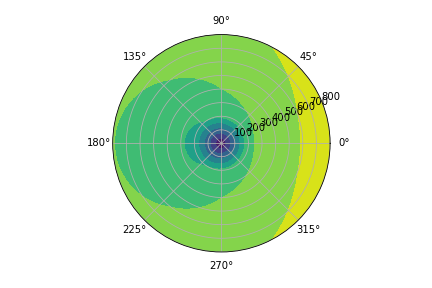
\includegraphics[scale=0.33]{pro1-1.png}
        \label{fig:pro1a-1}
    }
    \subfigure[m=2]{
        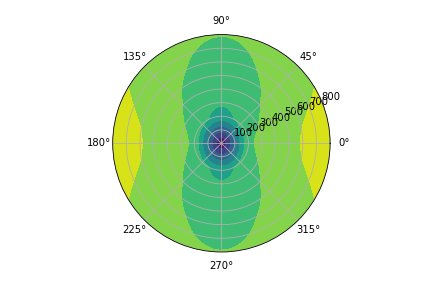
\includegraphics[scale=0.33]{pro1-2.png}
        \label{fig:pro1a-2} 
    }
    \subfigure[m=3]{
        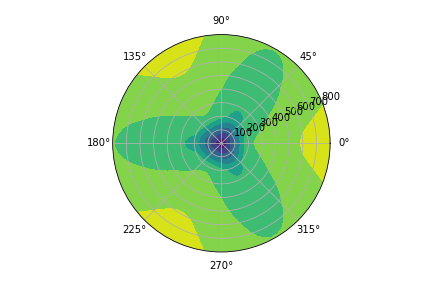
\includegraphics[scale=0.33]{pro1-3.png}
        \label{fig:pro1a-3} 
    }
    \caption{Draw the potential at t=0 for m=1,2,3}
    \label{fig:pro1a}
\end{figure}
% %-------------------------------

Before we do the following problems, we should first derive the mechanism of polar coordinate and the relation between potential, force and acceleration.

In polar coordinate, the equation can divide into two parts (r \& $\theta$):

\begin{equation}
    \vec{r}=r\hat{r}
    \label{eq:r}
\end{equation}

\begin{equation}
    \frac{d\vec{r}}{dt}=\dot{r}\hat{r}+r\dot{\theta} \hat{\theta}
    \label{eq:vr}
\end{equation}

\begin{equation}
    \frac{d^2\vec{r}}{dt^2}=(\ddot{r}-r\dot{\theta^2})\hat{r}+(2\dot{r}\dot{\theta}+r\ddot{\theta})\hat{\theta}
    \label{eq:ar}
\end{equation}

And the force provided by the potential can be gotten by the gradient of the potential (Eq.\ref{eq:potential}), and also divided into two parts (r \& $\theta$):

\begin{equation}
    F=F_r\hat{r}+F_{\theta}\hat{\theta}
     =-\bigtriangledown \Phi
     =-(\frac{\partial \Phi}{\partial r}\hat{r}+\frac{1}{r}\frac{\partial \Phi}{\partial \theta}\hat{\theta})
     \label{eq:F}
\end{equation}

\begin{equation}
    F_r=-\frac{v_{c}^{2}}{r}(1+\epsilon cos(m(\theta -\Omega_{p}t)))
    \label{eq:Fr}
\end{equation}

\begin{equation}
    F_{\theta}=\frac{1}{r}v_{c}^{2}\epsilon mln(r)sin(m(\theta -\Omega_{p}t))
    \label{eq:Ft}
\end{equation}

When we do rk4 in update subroutine, the update will be r, $\dot{r}$, $\ddot{r}$ ; $\theta$, $\dot{\theta}$, $\ddot{\theta}$.

So relation between potential and rk4 update will be the transform of  $F_r\&F_{\theta}$, we can use Eq.\ref{eq:ar} form with Eq.\ref{eq:Fr} \& Eq.\ref{eq:Ft} to get $\ddot{r}$ and $\ddot{\theta}$.
$$\ddot{r}=F_r+r\dot{\theta^2}$$
$$\ddot{\theta}=\frac{F_{\theta}-2\dot{r}\dot{\theta}}{r}$$
\underline{\textbf{1b. Integrate a circular orbit \& 1c. Given a small radial kick}}
% %-------------------------------
\begin{figure}[h]
    \centering
    \subfigure[pro1b integrate a circular orbit]{
        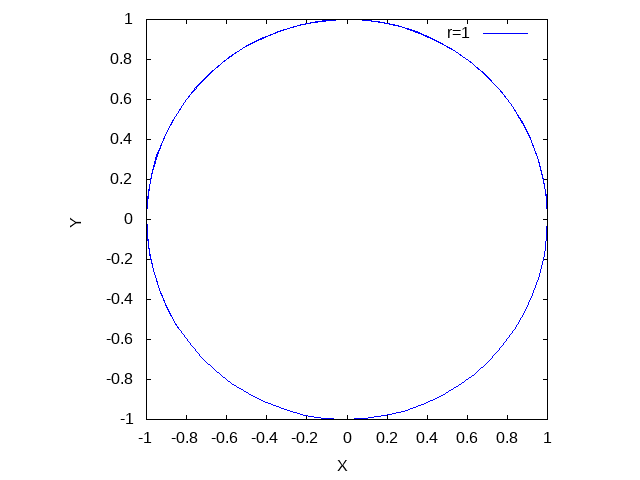
\includegraphics[scale=0.4]{pro1b.png}
        \label{fig:pro1b}
    }
    \subfigure[pro1c r(t) give a small radial kick]{
        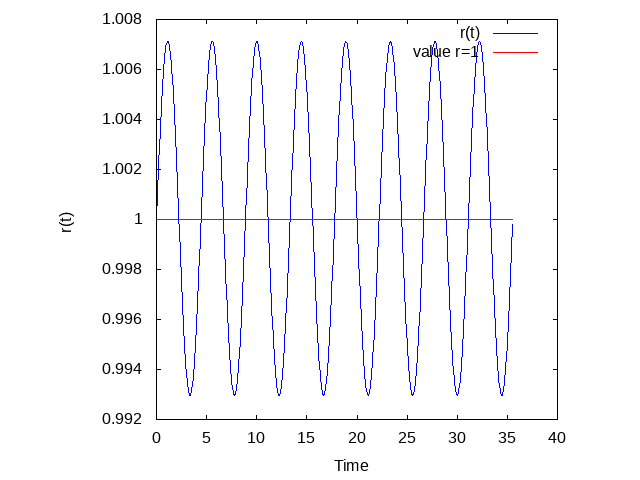
\includegraphics[scale=0.4]{pro1c.png}
        \label{fig:pro1c} 
    }
    \caption{pro1b \& pro1c figure}
    \label{fig:pro1bc}
\end{figure}
% %-------------------------------

In Fig.\ref{fig:pro1b}, we set r equal to 1 and test it by plot x-t plane.
Then we give a small radial kick ($v_r=0.01$), so the orbit seem to look like doing oscillation (Fig.\ref{fig:pro1c}) and will go back to initial position after $8\pi\kappa$, where $\kappa$ use the value $\sqrt{2}$ derive in the writing assignment Eq.\ref{eq:kappa}.
\\
\underline{\textbf{1d. Angular momentum L \& Energy E conservation}}
$$L=mr\omega^2$$
$$E=\frac{1}{2}mr^2\omega^2$$

Here I assume that m=1 and plot L(t) and E(t) and plot Fig.\ref{fig:pro1d} and also label the expect value as a red line in each figure.
Angular momentum has a good conservation, but energy will oscillate during period, I supposed that there is a error calculation during program run.\\
% %-------------------------------
\begin{figure}[h]
    \centering
    \subfigure[Angular momentum L(t)]{
        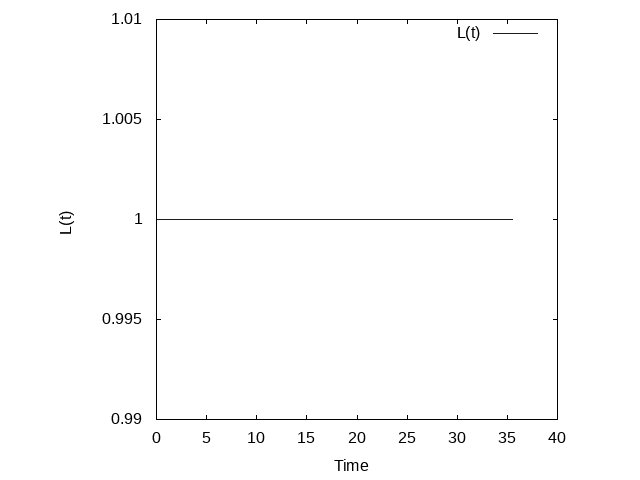
\includegraphics[scale=0.35]{pro1d_L.png}
        \label{fig:pro1d_L}
    }
    \subfigure[Energy E(t)]{
        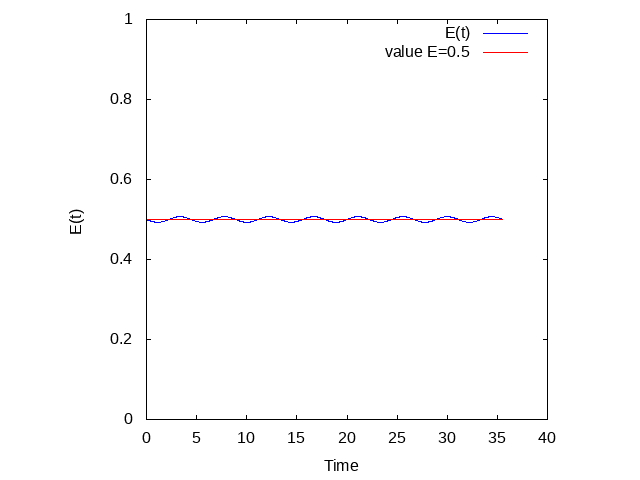
\includegraphics[scale=0.35]{pro1d_E2.png}
        \label{fig:pro1d_E} 
    }
    \caption{conservation discussion of given a small radial kick}
    \label{fig:pro1d}
\end{figure}
% %-------------------------------

\underline{\textbf{1e. Weak bar}}

Turn the potential form to weak bar with $\epsilon=0.02$ and $\omega_p=1.5$
We can see Fig.\ref{fig:pro1d_L} that the angular moment is obviously less than the expected value(L=1) ,and both of L and E have a broken wave form in each period. This may can explain L and E are not conserved in weak bar mode. \\
% %-------------------------------
\begin{figure}[h]
    \centering
    \subfigure[Angular momentum L(t)]{
        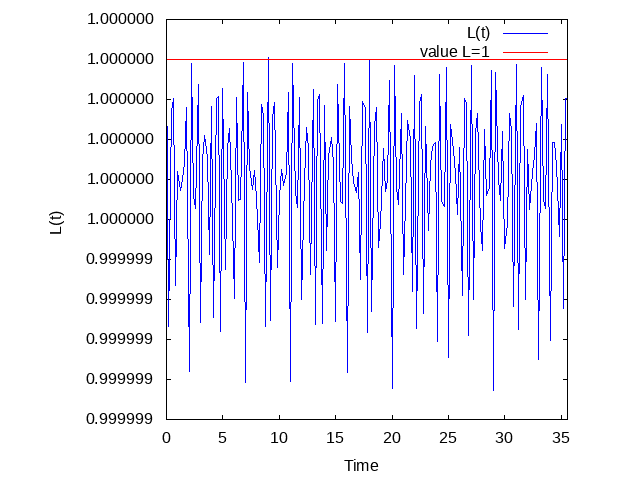
\includegraphics[scale=0.35]{pro1e_L2.png}
        \label{fig:pro1e_L}
    }
    \subfigure[Energy E(t)]{
        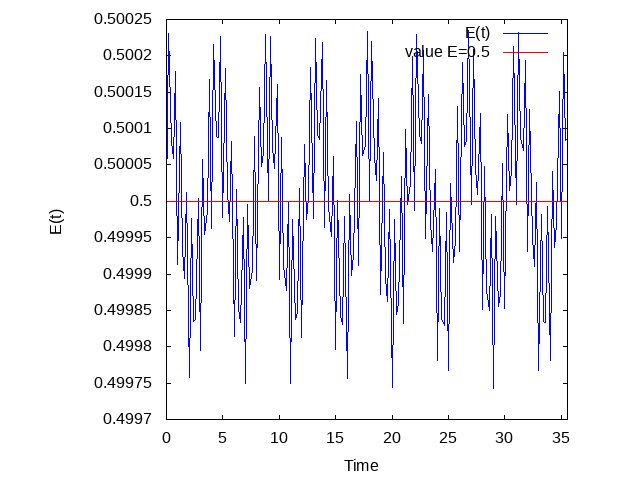
\includegraphics[scale=0.35]{pro1e_E2.png}
        \label{fig:pro1e_E} 
    }
    \caption{conservation discussion of weak bar}
    \label{fig:pro1e}
\end{figure}
% %-------------------------------

\underline{\textbf{1f. Discussion the epicyclic amplitude}}

$$H_J=E-\Omega_pL$$
The result of Jacobi integral compare to the initial value($H_J(0)$) seem to be the same(Fig.\ref{fig:pro1f}). Although they have the same oscillated action as a small radial kick (Fig.\ref{fig:pro1c}), but the non-conserved angular moment make the r(t) diverge and broken.
% %-------------------------------
\begin{figure}[h]
    \centering
    \subfigure[Jacobi integral $H_{j}$]{
        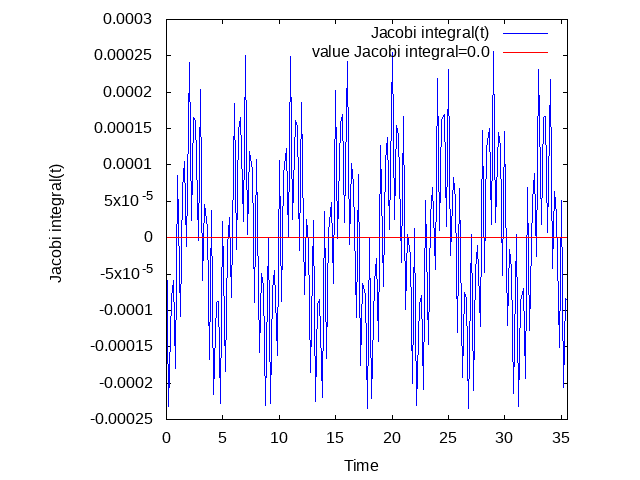
\includegraphics[scale=0.35]{pro1e2.png}
        \label{fig:pro1e_J}
    }
    \subfigure[r(t)]{
        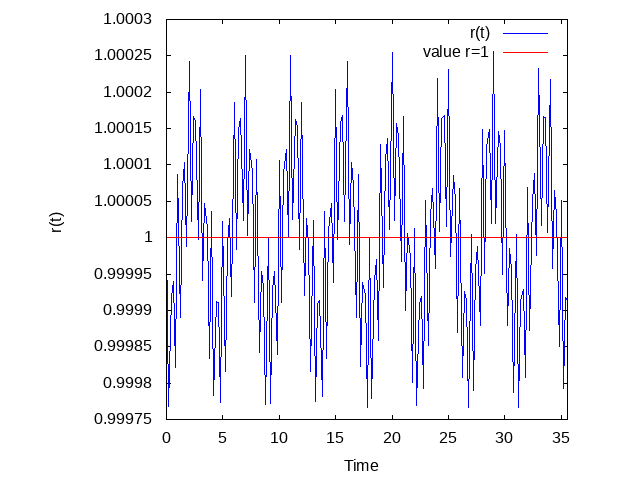
\includegraphics[scale=0.35]{pro1f1.png}
        \label{fig:pro1f} 
    }
    \caption{Jacobi integral $H_{j}$ \& r(t)}
    \label{fig:pro1ef}
\end{figure}
% %-------------------------------

\end{document}

% \footnote{Lagrangian point:\href{https://en.wikipedia.org/wiki/Lagrange\_point}{https://en.wikipedia.org/wiki/Lagrange\_point}}


% %-------------------------------
% \begin{figure}[h]
%     \centering 
% 	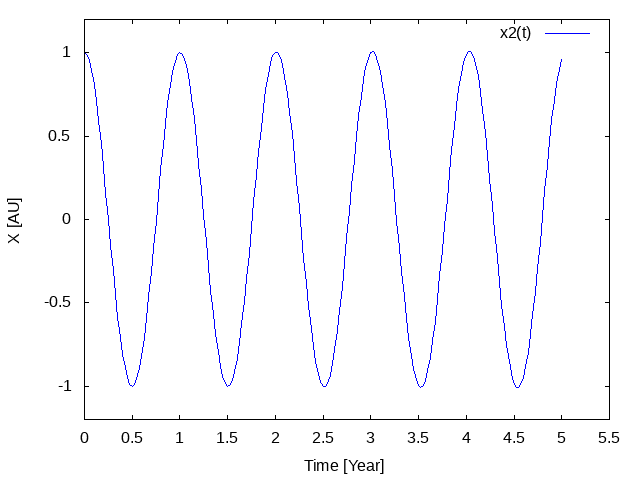
\includegraphics[scale=0.45]{pro1_x2.png}
% 	\caption{The trajectory of $m_1$ $m_2$ (when $m_2$ has a 1.25 factor of velocity).} %圖片註解
% 	\label{fig.pro1} %label 用這個就可以引用文章當中
% \end{figure}
% %-------------------------------

% %-------------------------------
% \begin{figure}[h]
%     \centering
%     \subfigure[dt=0.01yr]{
%         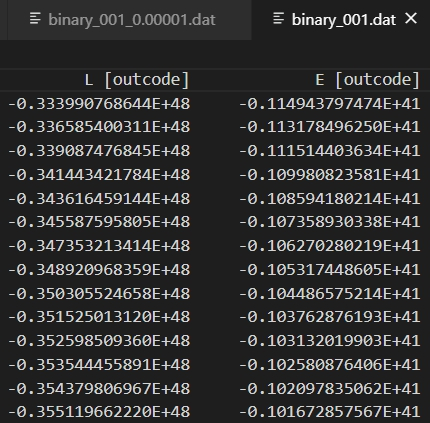
\includegraphics[scale=0.33]{01.jpg}
%         \label{01}
%     }
%     \subfigure[dt=0.001yr]{
%         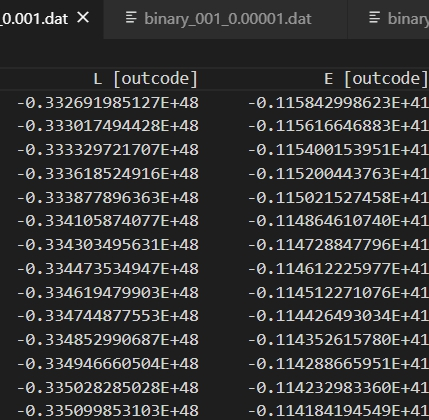
\includegraphics[scale=0.33]{001.jpg}
%         \label{001} 
%     }
%     \subfigure[dt=0.00001yr]{
%         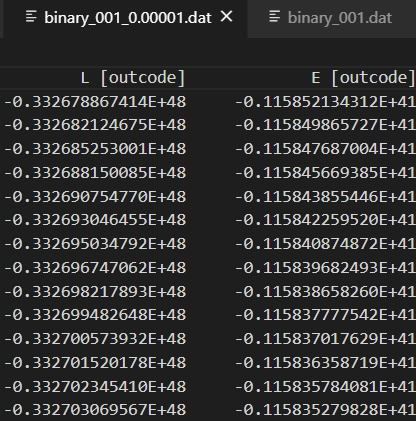
\includegraphics[scale=0.33]{00001.jpg}
%         \label{00001} 
%     }
%     \caption{L \& E in 0.01,0.001,0.00001 time step}
%     \label{fig:2c_dat}
% \end{figure}
% %-------------------------------
